
%(BEGIN_QUESTION)
% Copyright 2006, Tony R. Kuphaldt, released under the Creative Commons Attribution License (v 1.0)
% This means you may do almost anything with this work of mine, so long as you give me proper credit

A manometer may be used to measure differential pressure across a restriction placed within a pipe.  Pressure will be dropped as a result of flow through the pipe, making the manometer capable of (indirectly) measuring flow:

$$\includegraphics[width=15.5cm]{i00796x01.eps}$$

In the example shown above, the fluid moving through the pipe is air, and the manometer uses mercury as the indicating liquid.  If we try to measure the flow rate of a {\it liquid} such as water using the same technique, though, we will find that the manometer does not register quite the way we might expect:

$$\includegraphics[width=15.5cm]{i00796x02.eps}$$

That is to say, given the exact same amount of differential pressure generated by the restriction, the manometer will register differently than if it was measuring air pressure.  Determine whether the manometer will register falsely high or falsely low, and also {\it why} it will do so.

\underbar{file i00796}
%(END_QUESTION)





%(BEGIN_ANSWER)

The manometer will register falsely high, showing greater differential pressure than what is actually there.  If you are having difficulty figuring this out, imagine if the liquid moving through the pipe was just as dense as the mercury within the manometer: what would {\it that} do to the mercury in the manometer given any applied $\Delta$P?  In other words, set up a {\it thought experiment} with absurdly (simple) conditions and then look for patterns or trends which you may generalize for any condition.

\vskip 10pt

Challenge question: derive a mathematical correction factor for interpreting the manometer's indication to yield true inches of mercury $\Delta$P.

%(END_ANSWER)





%(BEGIN_NOTES)

Keep in mind that the water inside the manometer tubes (above the mercury) possesses weight, and generates a ``head'' just as the columns of mercury do!

%INDEX% Measurement, pressure: manometer across an orifice

%(END_NOTES)


